%%%%%%%%%%%%%%%%%%%%%%%%%%%%%%%%%%%%%%%%%
% "ModernCV" CV and Cover Letter
% LaTeX Template
% Version 1.1 (9/12/12)
%
% This template has been downloaded from:
% http://www.LaTeXTemplates.com
%
% Original author:
% Xavier Danaux (xdanaux@gmail.com)
%
% License:
% CC BY-NC-SA 3.0 (http://creativecommons.org/licenses/by-nc-sa/3.0/)
%
% Important note:
% This template requires the moderncv.cls and .sty files to be in the same
% directory as this .tex file. These files provide the resume style and themes
% used for structuring the document.
%
%%%%%%%%%%%%%%%%%%%%%%%%%%%%%%%%%%%%%%%%%
% 最后更新:2014年10月11日
%----------------------------------------------------------------------------------------
%   PACKAGES AND OTHER DOCUMENT CONFIGURATIONS
%----------------------------------------------------------------------------------------

\documentclass[10pt,a4paper,sans]{moderncv} % Font sizes: 10, 11, or 12; paper sizes: a4paper, letterpaper, a5paper, legalpaper, executivepaper or landscape; font families: sans or roman
% moderncv version 1.5.1 (29 Apr 2013)

\moderncvstyle{banking} % CV theme - options include: 'casual' (default), 'classic', 'oldstyle' and 'banking'
\moderncvcolor{black} % CV color - options include: 'blue' (default), 'orange', 'green', 'red', 'purple', 'grey' and 'black'
\usepackage[noindent]{ctex} %中文支持
% \setCJKmainfont{Libian SC}
\setCJKmainfont{HannotateSC-W5}

%\usepackage{lipsum} % Used for inserting dummy 'Lorem ipsum' text into the template

\usepackage[top=1cm,bottom=1.5cm,left=2cm,right=2cm]{geometry} % Reduce document margins
%\setlength{\hintscolumnwidth}{3cm} % Uncomment to change the width of the dates column
%\setlength{\makecvtitlenamewidth}{10cm} % For the 'classic' style, uncomment to adjust the width of the space allocated to your name

\usepackage{graphicx}

%----------------------------------------------------------------------------------------
%   NAME AND CONTACT INFORMATION SECTION
%----------------------------------------------------------------------------------------
\name{罗}{敏}
% All information in this block is optional, comment out any lines you don't need
\title{个人简历}
\address{长沙理工大学}{长沙, 湖南}
\phone[mobile]{(+86)~156~16039187}
\email{luomin5417@gmail.com}
\homepage{romix5417.github.io}
%\social[twitter]{username}
\social[github]{romix5417}
%\extrainfo{additional information}
%\photo[70pt][0.4pt]{photo} % The first bracket is the picture height, the second is the thickness of the frame around the picture (0pt for no frame)
%\quote{"A witty and playful quotation" - John Smith}

%----------------------------------------------------------------------------------------

\begin{document}

\makecvtitle % Print the CV title

%----------------------------------------------------------------------------------------
%   POSITION APPLIED(CAREER OBJECTIVE)
%----------------------------------------------------------------------------------------
\section{求职意向}
%\subsection{求职意向}
\cventry{期望月薪:  面议}{应聘职位:高级嵌入式软件工程师}{}{}{}{}


%----------------------------------------------------------------------------------------
%   SKill Set
%----------------------------------------------------------------------------------------

\section{我的技术栈}
\begin{center}
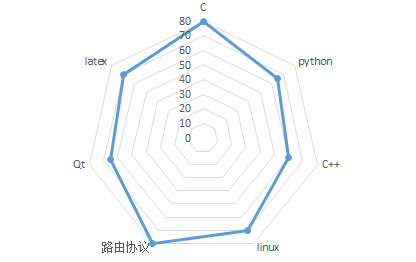
\includegraphics[width=0.5\linewidth]{myskillset.png}    
\end{center}

  
%----------------------------------------------------------------------------------------
%   EDUCATION SECTION
%----------------------------------------------------------------------------------------

\section{教育背景}

\cventry{2007---2011}{电子信息工程}{长沙理工大学}{本科}{}{}{\textit{GPA: 4.5/5(相当于百分制90分)}、工学学士}  % Arguments not required can be left empty

%----------------------------------------------------------------------------------------
%   WORK EXPERIENCE SECTION
%----------------------------------------------------------------------------------------

\section{项目经历}
%------------------------------------------------
\subsection{宽带无线自组网通信系统 (湖南宜通华盛科技有限公司)}

\cventry{2016.07---现在}{软件方面负责人}{}{}{}{
\begin{itemize}
\setlength{\itemindent}{2em}
    \item 嵌入式通信系统方案设计
    \item 嵌入式系统移植,主要包括Linux系统、Android系统、openwrt系统,rt-thread系统
    \item 自组网通信路由协议移植和组网算法改进,主要涉及到olsr协议和aodv协议等
    \item 使用Qt进行自组网通信设备的网络管理软件设计和代码编写
    \item 基于NXP的imx6q+ar9344芯片开发自组网移动通信设备,主要负责Linux系统和opemwrt系统移植
    \item imx6平台音频采集芯片,视频采集芯片,WIFI/蓝牙芯片,重力芯片感应,网卡芯片等驱动调试
    \item 基于海思hi3516D芯片进行网络摄像头的开发,基于海思平台实现了音视频采集和存储
    \item 基于全志a83t芯片的自组网iPad设备开发,主要涉及显示屏驱动的调试和触摸屏驱动调试、摄像头驱动调试
%    \item 推行Go在政府到普及
\end{itemize}
}




%%------------------------------------------------
\subsection{空间微星路由器 (国防科学技术大学网络研究所)}

\cventry{2015.09---2016.06}{项目重要成员}{}{}{}{
\begin{itemize}
\setlength{\itemindent}{2em}
    \item 基于am335x芯片的平台系统设计,SDRAM、eMMC等外设芯片选型,am335x芯片连接外设管脚分配
    \item 基于新开发平台uboot修改和移植
    \item 基于新开发平台的linux操作系统移植 
    \item 基于am335x芯片外接设备的调试和驱动修改,主要有SDRAM调试,eMMc驱动调试,网络接口驱动调试
\end{itemize}
}


%%------------------------------------------------
\subsection{基于标地分离的空间网络通信设备接入协议设计 (国防科学技术大学网络研究所)}

\cventry{2015.01---2015.08}{项目主要成员}{}{}{}{
\begin{itemize}
\setlength{\itemindent}{2em}
    \item 主要负责整个协议设计,地面注册模块,数据转发模块,网关与映射服务器交互注册保活模块等的代码编写
    \item 编写地面设备接入注册模块,映射服务器模块,数据转发模块代码
    \item 编写基于tunel隧道技术的IP报文封装模块,网关与映射服务器交互注册保活模块
\end{itemize}
}


%%------------------------------------------------
\subsection{空间路由协议设计与代码编写 (国防科学技术大学网络研究所)}

\cventry{2013.12---2014.12}{项目重要成员}{}{}{}{
\begin{itemize}
\setlength{\itemindent}{2em}
    \item 主要负责预制路由协议的框架设计和各个模块的代码编写工作
    \item 预制路由配置文件解析模块、路由管理模块、同步路由预制管理模块、预制路由校验模块
    \item 协议验证与仿真等工作 
\end{itemize}
}
%%------------------------------------------------

%%------------------------------------------------
\subsection{空间路由器报文转发平面设计处理 (国防科学技术大学网络研究所)}

\cventry{2012.12---2013.12}{项目重要成员}{}{}{}{
\begin{itemize}
\setlength{\itemindent}{2em}
    \item 基于SPARCv8架构BM3803芯片组的vxWorks系统移植于协议栈调试
    \item 报文收发模块、FIB表项下发模块、ARP表项下发模块、接口驱动模块代码编写 
    \item SpaceWire总线驱动模块代码编写
    \item FIB表项下发和ARP表项下发模块、报文收发模块的代码设计和编写工作
\end{itemize}
}
%%------------------------------------------------
%----------------------------------------------------------------------------------------
%   AWARDS SECTION
%----------------------------------------------------------------------------------------

\section{荣誉奖励}
\cvitem{2018.1}{湖南宜通华盛科技有限公司优秀员工}
\cvitem{2015.2}{国防科大六院优秀员工}

%----------------------------------------------------------------------------------------
%   AWARDS SECTION
%----------------------------------------------------------------------------------------

\section{个人爱好}
\cvitem{体育运动}{足球,篮球,乒乓球,羽毛球}
\cvitem{科技}{阅读科技类博客,写博客}
\cvitem{开源项目}{乐于在github上参与各种开源软件开发和贡献代码}


\section{语言}
\cvitem{英语}{能够熟练快速阅读各种英文参考文献和技术手册}
\end{document}
